\documentclass{article}
\usepackage[utf8]{inputenc}
\usepackage{amsmath}
\usepackage{amssymb}
\usepackage{amsthm}
\usepackage{tikz}
\setlength{\parindent}{0pt}

\newtheorem*{theorem}{Theorem}
\newtheorem*{definition}{Definition}
\newtheorem*{lemma}{Lemma}
\newtheorem*{corollary}{Corollary}
\newtheorem{example}{Example}

\title{Problem Set 1}
\author{}
\date{}

\begin{document}

\begin{center}
{\rmfamily\bfseries\Large 18.02 EXERCISES}

\vspace{25px}

{\rmfamily\bfseries\LARGE Problem Set 1: Vectors, Determinants and Planes}
\end{center}

\begin{center}
\section*{Part I}
\end{center}

\subsection*{Unit 1 Vectors}

1. Find the magnitude and direction of the vectors \\
a) $\vec{i} + \vec{j} + \vec{k}$ \\
b) $2\vec{i} - \vec{j} + 2\vec{k}$ \\
c) $3\vec{i} - 6\vec{j} - 2\vec{k}$

Solution:

a) Suppose $\vec{A} = \vec{i} + \vec{j} + \vec{k}$, then
\[
  \begin{split}
    |\vec{A}| &= \sqrt{1^2 + 1^2 + 1^2} \\
              &= \sqrt{3}
  \end{split}
\]
\[
  \begin{split}
    dir \vec{A} &= \frac{\vec{A}}{|\vec{A}|} \\
                &= \frac{\vec{i} + \vec{j} + \vec{k}}{\sqrt{3}} \\
                &= \frac{\sqrt{3}}{3}\vec{i} + \frac{\sqrt{3}}{3}\vec{j} + \frac{\sqrt{3}}{3}\vec{k}
  \end{split}
\]

b) Suppose $\vec{A} = 2\vec{i} - \vec{j} + 2\vec{k}$, then
\[
  \begin{split}
    |\vec{A}| &= \sqrt{2^2 + (-1)^2 + 2^2} \\
              &= \sqrt{9} \\
              &= 3
  \end{split}
  |\vec{A}| = \sqrt{2^2 + (-1)^2 + 2^2} = \sqrt{9} = 3
\]
\[
  \begin{split}
    dir \vec{A} &= \frac{\vec{A}}{|\vec{A}|} \\
                &= \frac{2\vec{i} - \vec{j} + 2\vec{k}}{3} \\
                &= \frac{2}{3}\vec{i} - \frac{1}{3}\vec{j} + \frac{2}{3}\vec{k}
  \end{split}
\]

c) Suppose $\vec{A} = 3\vec{i} - 6\vec{j} - 2\vec{k}$, then
\[
  \begin{split}
    |\vec{A}| &= \sqrt{3^2 + (-6)^2 + (-2)^2} \\
              &= \sqrt{49} \\
              &= 7
  \end{split}
\]
\[
  \begin{split}
    dir \vec{A} &= \frac{\vec{A}}{|\vec{A}|} \\
                &= \frac{3\vec{i} - 6\vec{j} - 2\vec{k}}{7} \\
                &= \frac{3}{7}\vec{i} - \frac{6}{7}\vec{j} - \frac{2}{7}\vec{k}
  \end{split}
\]

2. a) Let $P$ and $Q$ be two points in space, and X the midpoint of the line
segment $PQ$. Let $O$ be an arbitrary fixed point; show that as vectors, $OX =
\frac{1}{2}(OP + OQ)$.\\
b) With the notation of part (a), assume that X divides the line segment $PQ$
in the ratio $r:s$, where $r + s = 1$. Derive an expression for $OX$ in terms
of $OP$ and $OQ$.

Solution:

a) Suppose $P = (a_1, b_1, c_1)$, $Q = (a_2, b_2, c_2)$, and $O = (a_0, b_0, c_0)$.\\
Since $X$ is the midpoint of the line segment $PQ$, then
\[
    X = (\frac{a_1 + a_2}{2}, \frac{b_1 + b_2}{2}, \frac{c_1 + c_2}{2})
\]
Therefore,
\[
  \vec{OP} = <a_1 - a_0, b_1 - b_0, c_1 - c_0>
\]
\[
  \vec{OQ} = <a_2 - a_0, b_2 - b_0, c_2 - c_0>
\]
\[
  \begin{split}
    \vec{OX} &= <\frac{a_1 + a_2}{2} - a_0, \frac{b_1 + b_2}{2} - b_0, \frac{c_1 + c_2}{2} - c_0> \\
             &= \frac{1}{2}<a_1 + a_2 - 2a_0, b_1 + b_2 - 2b_0, c_1 + c_2 - 2c_0> \\
             &= \frac{1}{2}(\vec{OP} + \vec{OQ})
  \end{split}
\]

b) Since $X$ divides the line segment $PQ$ in the ratio $r : s$, where
$r + s = 1$,
\[
  \vec{PX} = \frac{r}{r + s}\vec{PQ}
\]
Then we also know
\[
  \vec{PQ} = \vec{OQ} - \vec{OP}
\]
\[
  \vec{OX} = \vec{OP} + \vec{PX}
\]
Therefore,
\[
  \begin{split}
    \vec{OX} &= \vec{OP} + \vec{PX} \\
             &= \vec{OP} + \frac{r}{r + s}\vec{PQ} \\
             &= \vec{OP} + \frac{r}{r + s}(\vec{OQ} - \vec{OP}) \\
             &= \frac{s}{r + s}\vec{OP} + \frac{r}{r + s}\vec{OQ} \\
  \end{split}
\]

3. What are the $\vec{i} \vec{j}$-components of a plane vector $\vec{A}$ of
length 3, if it makes an angle of $30^{\circ}$ with $\vec{i}$ and $60^{\circ}$
with $\vec{j}$. Is the second condition redundant?

Solution:

\begin{tikzpicture}
  [help lines/.style={dashed}]
  \draw[->] (-3, 0, 0) -- (3, 0, 0) node[anchor=south] {x};
  \draw[->] (0, 0, 0) -- (1, 0, 0) node[anchor=south] {$\vec{i}$};
  \draw[->] (0, -3, 0) -- (0, 3, 0) node[anchor=east] {y};
  \draw[->] (0, 0, 0) -- (0, 1, 0) node[anchor=east] {$\vec{j}$};
  \draw[->] (0, 0, 0) -- (2.6, 1.5, 0) node[anchor=south] {$\vec{A}$};
  \draw (0.2, 0) arc [start angle=0, end angle=30, radius=0.2] 
    node[anchor=west] {$30^{\circ}$};
  \draw[->, help lines] (0, 0, 0) -- (2.6, -1.5, 0) node[anchor=north] {$\vec{A'}$};
\end{tikzpicture}

Apparently
\[
  \begin{split}
    \vec{A} &= <|\vec{A}|\cos(30^{\circ}), |\vec{A}|\sin(30^{\circ})> \\
            &= <3 \cdot \frac{\sqrt{3}}{2}, 3 \cdot \frac{1}{2}> \\
            &= <\frac{3\sqrt{3}}{2}, \frac{3}{2}> \\
            &= \frac{3\sqrt{3}}{2}\vec{i} + \frac{3}{2} \vec{j} \\
  \end{split}
\]
The second condition that the vector $\vec{A}$ makes an angle of $60^{\circ}$
with $\vec{j}$ is not redundant, otherwise the referred vector can be $\vec{A}$
or $\vec{A'}$ in the above diagram.

4. A small plane wishes to fly due north at 200 mph (as seen from the ground),
in a wind blowing from the northeast at 50 mph. Tell with what vector velocity
in the air it should travel (given the $\vec{i} \vec{j}$-components).

Solution:

Suppose that $\vec{i}$ represents east, then $\vec{j}$ represents north, and
$-\vec{i}$ represents west, and $-\vec{j}$ represents south. Let $\vec{V_w}$
denote the velocity of the wind, $\vec{V_p}$ denote the velocity of the plane in
the air, and $\vec{V}$ denote the velocity of plane seen from the ground. \\
$\vec{V}$ should be the result of $\vec{V_p}$ and $\vec{V_w}$ applied together,
therefore
\[
  \vec{V} = \vec{V_p} + \vec{V_w}
\]
According to the problem description,
\[
  \begin{split}
    \vec{V_w} &= <50\cos45^{\circ}, 50\sin45^{\circ}> \\
              &= <25\sqrt{2}, 25\sqrt{2}> \\
  \end{split}
\]
\[
  \vec{V} = <0, 200>
\]
Therefore
\[
  \begin{split}
    \vec{V_p} &= \vec{V} - \vec{V_w} \\
              &= <0, 200> - <25\sqrt{2}, 25\sqrt{2}> \\
              &= <-25\sqrt{2}, 200 - 25\sqrt{2}> \\
  \end{split}
\]

5. Let $\vec{A} = a \vec{i} + b \vec{j}$ be a plane vector; find in terms of
$a$ and $b$ the vectors $\vec{A'}$ and $\vec{A''}$ resulting from rotating
$\vec{A}$ by $90^{\circ}$ \hspace{10px} a) clockwise \hspace{10px} b)
counterclockwise.\\
c) Let $\vec{i'} = (3 \vec{i} + 4 \vec{j}) / 5$. Show that $\vec{i'}$ is a unit
vector, and use the first part of the exercise to find a vector $\vec{j'}$ such
that $\vec{i'}$, $\vec{j'}$ forms a right-handed coordinate system.

Solution:

a) According to the problem description, $\vec{A'}$ is the result of rotating
$\vec{A}$ clockwise by $90^{\circ}$. Therefore, the $\vec{i} \vec{j}$-components
of $\vec{A}$ should be rotated the same way to get the corresponding components
of $\vec{A'}$. After being rotated in the mentioned way, $\vec{i}$ becomes
$-\vec{j}$, and $\vec{j}$ becomes $\vec{i}$. Therefore,
\[
  \vec{A'} = b \cdot \vec{i} - a \cdot \vec{j}
\]

b) Similar to a), after being rotated counterclockwise by $90^{\circ}$,
$\vec{i}$ becomes $\vec{j}$, and $\vec{j}$ becomes $-\vec{i}$. Therefore,
\[
  \vec{A''} = -b \cdot \vec{i} + a \cdot \vec{j}
\]

c) To prove $\vec{i'}$ is a unit vector,
\[
  \begin{split}
    |\vec{i'}| &= \sqrt{(\frac{3}{5})^2 + (\frac{4}{5})^2} \\
               &= 1
  \end{split}
\]
To form a right-handed coordinate system, $\vec{j'}$ should be the result of
rotating $\vec{i'}$ counterclockwise by $90^{\circ}$. According the part b),
we can derive that
\[
  \vec{j'} = -\frac{4}{5} \cdot \vec{i} + \frac{3}{5} \cdot \vec{j}
\]

6. The direction of a space vector is in engineering practice often given by
its \textbf{direction cosines}. To describe these, let 
$\vec{A} = a \vec{i} + b \vec{j} + c \vec{k}$ be a space vector, represented as 
an origin vector, and let $\alpha$, $\beta$, and $\gamma$ be the three angles 
($\le \pi$) that $\vec{A}$ makes respectively with $\vec{i}$, $\vec{j}$, and 
$\vec{k}$.\\
a) Show that $dir \vec{A} = \cos\alpha \vec{i} + \cos\beta \vec{j} +
\cos\gamma \vec{k}$. (The three coefficients are called the \emph{direction
cosines} of $\vec{A}$.)\\
b) Express the direction cosines of $\vec{A}$ in terms of $a$, $b$, $c$; find
the direction cosines of the vector $-\vec{i} + 2\vec{j} + 2\vec{k}$.\\
c) Prove that three numbers $t$, $u$, $v$ are the direction cosines of a vector
in space if and only if they satisfy $t^{2} + u^{2} + v^{2} = 1$.

Solution:

a) According to the definition, $dir \vec{A}$ is the unit vector with the same
direction as $\vec{A}$, hence $dir \vec{A}$ makes the same angles with
$\vec{i}$, $\vec{j}$, $\vec{k}$ as $\vec{A}$, i.e. $\alpha$, $\beta$, and 
$\gamma$ respectively. Then according to the definition of component vectors, 
i.e. the cast on a specific directions, we can derive that
\[
  dir \vec{A} = \cos\alpha \cdot \vec{i} + \cos\beta \cdot \vec{j} + \cos\gamma \cdot \vec{k}
\]

b) According to the definition of vector directions, 
\[
  \begin{split}
    dir \vec{A} &= \frac{\vec{A}}{|\vec{A}|} \\
                &= \frac{a \vec{i} + b \vec{j} + c \vec{k}}{\sqrt{a^2 + b^2 + c^2}} \\
                &= \frac{a}{\sqrt{a^2 + b^2 + c^2}} \vec{i} + \frac{b}{\sqrt{a^2 + b^2 + c^2}} \vec{j} + \frac{c}{\sqrt{a^2 + b^2 + c^2}} \vec{k} \\
                &= \cos\alpha \cdot \vec{i} + \cos\beta \cdot \vec{j} + \cos\gamma \cdot \vec{k}
  \end{split}
\]
Therefore,
\begin{gather*}
  \cos\alpha = \frac{a}{\sqrt{a^2 + b^2 + c^2}} \\
  \cos\beta = \frac{b}{\sqrt{a^2 + b^2 + c^2}} \\
  \cos\gamma = \frac{c}{\sqrt{a^2 + b^2 + c^2}} \\
\end{gather*}
Hence for the vector $-\vec{i} + 2\vec{j} + 2\vec{k}$,
\begin{gather*}
  \begin{split}
    \cos\alpha &= \frac{-1}{\sqrt{(-1)^2 + 2^2 + 2^2}} \\
               &= -\frac{1}{3} \\
  \end{split} \\
  \begin{split}
    \cos\beta &= \frac{2}{\sqrt{(-1)^2 + 2^2 + 2^2}} \\
              &= \frac{2}{3} \\
  \end{split} \\
  \begin{split}
    \cos\gamma &= \frac{2}{\sqrt{(-1)^2 + 2^2 + 2^2}} \\
              &= \frac{2}{3} \\
  \end{split} \\
\end{gather*}

c) Proof: \\
If $t$, $u$, $v$ are the direction cosines of a vector $\vec{A}$ in space, then 
they are the components of its direction:
\[
  dir \vec{A} = t \cdot \vec{i} + u \cdot \vec{j} + v \cdot \vec{k}
\]
Since $dir \vec{A}$ is a unit vector, then
\[
  |dir \vec{A}| = \sqrt{t^2 + u^2 + v^2} = 1
\]
\[
  t^2 + u^2 + v^2 = 1
\]
If $t$, $u$, $v$ satisfy $t^2 + u^2 + v^2 = 1$, then we can construct a unit 
vector $\vec{D} = t \cdot \vec{i} + u \cdot \vec{j} + v \cdot \vec{k}$. Then 
$t$, $u$, $v$ are the direction cosines of the constructed space vector.

7. Prove using vector methods (without components) that the line segment
joining the midpoints of two sides of a triangle is parallel to the third side
and half its length. (Call the two sides $\vec{A}$ and $\vec{B}$.)

Proof:

Suppose that the two sides are $\vec{A}$ and $\vec{B}$, the third side is 
$\vec{C}$, and the line segment joining the midpoints of the two sides is
$\vec{C'}$. Then
\[
  \vec{C} = \vec{A} - \vec{B}
\]
or
\[
  \vec{C} = -(\vec{A} - \vec{B})
\]
And
\[
  \begin{split}
    \vec{C'} &= \frac{1}{2}\vec{A} - \frac{1}{2}\vec{B} \\
             &= \frac{1}{2}(\vec{A} - \vec{B}) \\
  \end{split}
\]
or
\[
  \begin{split}
    \vec{C'} &= -(\frac{1}{2}\vec{A} - \frac{1}{2}\vec{B}) \\
             &= -\frac{1}{2}(\vec{A} - \vec{B}) \\
  \end{split}
\]
Therefore, either of the following equations must hold:
\[
  \vec{C'} = \frac{1}{2}\vec{C}
\]
or
\[
  \vec{C'} = -\frac{1}{2}\vec{C}
\]
Therefore, $\vec{C'}$ is parallel to $\vec{C}$ and the magnitude of $\vec{C'}$ 
is the half of the one of $\vec{C}$.

8. Prove using vector methods (without components) that the diagonals of a
parallelogram bisect each other. (One way: let $X$ and $Y$ be the midpoints of
the two diagonals; show $X$ = $Y$.)

Proof:

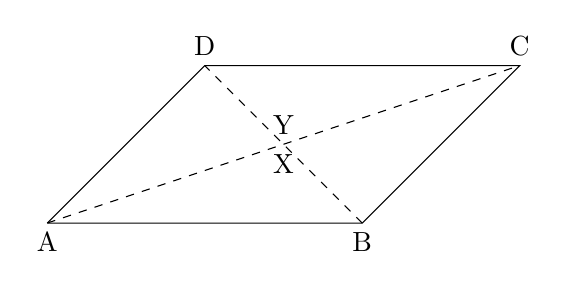
\begin{tikzpicture}
  [help lines/.style={dashed}]
  \draw[-] (-2, 0) node[anchor=north] {A} -- (2, 0) node[anchor=north] {B} -- 
    (4, 2) node[anchor=south] {C} -- (0, 2) node[anchor=south] {D} -- (-2, 0);
  \draw[-, help lines] (-2, 0) -- (1, 1) node[anchor=north] {X} -- (4, 2);
  \draw[-, help lines] (2, 0) -- (1, 1) node[anchor=south] {Y} -- (0, 2);
\end{tikzpicture}

As shown in the diagram, suppose that the four endpoints of a parallelogram are 
$A$, $B$, $C$, $D$, and the midpoint of the diagonal $AC$ is $X$, and the 
midpoint of the diagonal $BD$ is $Y$. Then
\[
  \begin{split}
    \vec{AX} &= \frac{1}{2}\vec{AC} \\
             &= \frac{1}{2}(\vec{AB} + \vec{AD}) \\
             &= \frac{1}{2}\vec{AB} + \frac{1}{2}\vec{AD} \\
  \end{split}
\]
\[
  \begin{split}
    \vec{AY} &= \vec{AB} + \vec{BY} \\
             &= \vec{AB} + \frac{1}{2}\vec{BD} \\
             &= \vec{AB} + \frac{1}{2}(\vec{AD} - \vec{AB}) \\
             &= \frac{1}{2}\vec{AB} + \frac{1}{2}\vec{AD} \\
  \end{split}
\]
Therefore, $\vec{AX} = \vec{AY}$, which means the midpoints of the two 
diagonals are the same point. Hence, the two diagonals of a parallelogram 
bisect each other.

\subsection*{Unit 2 Dot Product}

1. Tell for what values of $c$ the vectors $c \vec{i} + 2 \vec{j} - \vec{k}$
and $\vec{i} - \vec{j} + 2 \vec{k}$ will \\
a) be orthogonal \hspace{10px} b) form an acute angle

Solution:

a) The vectors $c \vec{i} + 2 \vec{j} - \vec{k}$ and 
$\vec{i} - \vec{j} + 2 \vec{k}$ are orthogonal if and only if
\[
  (c \vec{i} + 2 \vec{j} - \vec{k}) \cdot (\vec{i} - \vec{j} + 2 \vec{k}) = 0
\]
\[
  c - 2 - 2 = 0
\]
\[
  c = 4
\]

b) The vectors $c \vec{i} + 2 \vec{j} - \vec{k}$ and 
$\vec{i} - \vec{j} + 2 \vec{k}$ form an acute angle if and only if
\[
  (c \vec{i} + 2 \vec{j} - \vec{k}) \cdot (\vec{i} - \vec{j} + 2 \vec{k}) > 0
\]
\[
  c - 2 - 2 > 0
\]
\[
  c > 4
\]

2. Using vectors, find the angle between a longest diagonal $PQ$ of a cube,
and \\
a) a diagonal $PR$ of one of its faces; \hspace{10px} b) an edge $PS$ of the
cube. \\
(Choose a size and position for the cube that makes calculation easiest.)

Solution:

a) Suppose that $P = (0, 0, 0)$, $Q = (1, 1, 1)$, and $R = (1, 1, 0)$. 
Therefore, $\vec{PQ} = <1, 1, 1>$, and $\vec{PR} = <1, 1, 0>$. Then, the angle
$\theta$ between $PQ$ and $PR$ satisfies
\[
  \begin{split}
    \cos\theta &= \frac{\vec{PQ} \cdot \vec{PR}}{|\vec{PQ}| \cdot |\vec{PR}|} \\
               &= \frac{1 \times 1 + 1 \times 1 + 1 \times 0}{\sqrt{1^2 + 1^2 + 1^2} \times \sqrt{1^2 + 1^2 + 0^2}} \\
               &= \frac{2}{\sqrt{3} \times \sqrt{2}} \\
               &= \frac{\sqrt{6}}{3} \\
  \end{split}
\]

b) Suppose that $P = (0, 0, 0)$, $Q = (1, 1, 1)$, and $S = (1, 0, 0)$. 
Therefore, $\vec{PQ} = <1, 1, 1>$, and $\vec{PS} = <1, 0, 0>$. Then, the angle
$\theta$ between $PQ$ and $PS$ satisfies
\[
  \begin{split}
    \cos\theta &= \frac{\vec{PQ} \cdot \vec{PS}}{|\vec{PQ}| \cdot |\vec{PS}|} \\
               &= \frac{1 \times 1 + 1 \times 0 + 1 \times 0}{\sqrt{1^2 + 1^2 + 1^2} \times \sqrt{1^2 + 0^2 + 0^2}} \\
               &= \frac{1}{\sqrt{3} \times 1} \\
               &= \frac{\sqrt{3}}{3} \\
  \end{split}
\]

3. Three points in space are $P:(a,1,-1)$, $Q:(0,1,1)$, $R:(a,-1,3)$. For what
value(s) of $a$ will $PQR$ be\\
a) a right angle \hspace{10px} b) an acute angle

Solution:

a) $PQR$ will be a right angle $\iff$ $\vec{PQ} \cdot \vec{QR} = 0$
\begin{gather*}
  \vec{PQ} = <-a, 0, 2> \\
  \vec{QR} = <a, -2, 2> \\
  \vec{PQ} \cdot \vec{QR} = 0 \\
  <-a, 0, 2> \cdot <a, -2, 2> = 0 \\
  -a^2 + 4 = 0 \\
  a = \pm 2 \\
\end{gather*}

b) $PQR$ will be an acute angle $\iff$ $\vec{PQ} \cdot \vec{QR} > 0$
\begin{gather*}
  \vec{PQ} \cdot \vec{QR} > 0 \\
  <-a, 0, 2> \cdot <a, -2, 2> > 0 \\
  -a^2 + 4 > 0 \\
  a^2 < 4 \\
  -2 < a < 2 \\
\end{gather*}

4. Find the component of the force $\vec{F} = 2 \vec{i} - 2 \vec{j} + \vec{k}$
in\\
a) the direction $\frac{\vec{i} + \vec{j} - \vec{k}}{\sqrt{3}}$ \hspace{10px}
b) the direction of the vector $3 \vec{i} + 2 \vec{j} - 6 \vec{k}$.

Solution:

a) To get the component of a vector along a certain direction, we can calculate 
the dot product of the vector and the direction. Since dot product satisfies the 
distributive property, the dot product of a vector and a direction is equivalent 
to the dot product of the direction and the component vector of the vector along 
the direction, plus the dot product of the direction and the other component 
vector, which is perpendicular to the direction. Therefore, the result is only 
the dot product of the direction and the component vector of the vector along 
the direction, which is the component value.
\begin{equation*}
\begin{split}
  c &= (2\vec{i} - 2\vec{j} + \vec{k}) \cdot (\frac{\vec{i} + \vec{j} - \vec{k}}{\sqrt{3}}) \\
    &= <2, -2, 1> \cdot <\frac{\sqrt{3}}{3}, \frac{\sqrt{3}}{3}, -\frac{\sqrt{3}}{3}> \\
    &= -\frac{\sqrt{3}}{3} \\
\end{split}
\end{equation*}

b) Similar to a),
\begin{gather*}
\begin{split}
  dir(3\vec{i} + 2\vec{j} - 6\vec{k}) &= \frac{3\vec{i} + 2\vec{j} - 6\vec{k}}{|3\vec{i} + 2\vec{j} - 6\vec{k}|} \\
                                      &= \frac{3\vec{i} + 2\vec{j} - 6\vec{k}}{7} \\
                                      &= <\frac{3}{7}, \frac{2}{7}, -\frac{6}{7}> \\
\end{split} \\
\begin{split}
  c &= (2\vec{i} - 2\vec{j} + \vec{k}) \cdot dir(3\vec{i} + 2\vec{j} - 6\vec{k}) \\
    &= <2, -2, 1> \cdot <\frac{3}{7}, \frac{2}{7}, -\frac{6}{7}> \\
    &= -\frac{4}{7} \\
\end{split} \\
\end{gather*}

5. Prove using vector methods (without components) that the diagonals of a
parallelogram have equal lengths if and only if it is a rectangle.

Proof:

Let $\vec{A}$ and $\vec{B}$ denote the vectors of two adjecent sides of a parallelogram,
and $\vec{D_1}$ and $\vec{D_2}$ denote the two diagonals of the parallelogram.
\begin{gather*}
  \vec{D_1} = \vec{A} + \vec{B} \\
  \vec{D_2} = \vec{A} - \vec{B} \\
\end{gather*}
The two diagonals have equal lengths is equivalent to
\begin{gather*}
  |\vec{D_1}| = |\vec{D_2}| \\
  \iff |\vec{A} + \vec{B}| = |\vec{A} - \vec{B}| \\
  \iff |\vec{A} + \vec{B}|^2 = |\vec{A} - \vec{B}|^2 \\
  \iff (\vec{A} + \vec{B}) \cdot (\vec{A} + \vec{B}) = (\vec{A} - \vec{B}) \cdot (\vec{A} - \vec{B}) \\
  \iff |\vec{A}|^2 + |\vec{B}|^2 + 2\vec{A} \cdot \vec{B} = |\vec{A}|^2 + |\vec{B}|^2 - 2\vec{A} \cdot \vec{B} \\
  \iff 4\vec{A} \cdot \vec{B} = 0 \\
  \iff \vec{A} \cdot \vec{B} = 0 \\
  \iff \vec{A} \perp \vec{B} \\
\end{gather*}
which is equivalent to the parallelogram is a rectangle.

Therefore, it is proved that the diagonals of a parallelogram have equal lengths 
if and only if it is a rectangle.

6. Prove using vector methods (without components) that the diagonals of a
parallelogram are perpendicular if and only if it is a rhombus, i.e., its four
sides are equal.

Proof:

Let $\vec{A}$ and $\vec{B}$ denote the vectors of two adjecent sides of a parallelogram,
and $\vec{D_1}$ and $\vec{D_2}$ denote the two diagonals of the parallelogram.
\begin{gather*}
  \vec{D_1} = \vec{A} + \vec{B} \\
  \vec{D_2} = \vec{A} - \vec{B} \\
\end{gather*}
The two diagonals are perpendicular is equivalent to 
\begin{gather*}
  \vec{D_1} \perp \vec{D_2} \\
  \iff \vec{D_1} \cdot \vec{D_2} = 0 \\
  \iff (\vec{A} + \vec{B}) \cdot (\vec{A} - \vec{B}) = 0 \\
  \iff |\vec{A}|^2 - |\vec{B}|^2 = 0 \\
  \iff |\vec{A}|^2 = |\vec{B}|^2 \\
  \iff |\vec{A}| = |\vec{B}| \\
\end{gather*}
which is equivalent to the four sides of the parallelogram are equal.

Therefore, it is proved that the diagonals of a parallelogram are perpendicular 
if and only if it is a rhombus, i.e., its four sides are equal.

7. Prove using vector methods (without components) that an angle inscribed in
a semicircle is a right angle.

Proof:

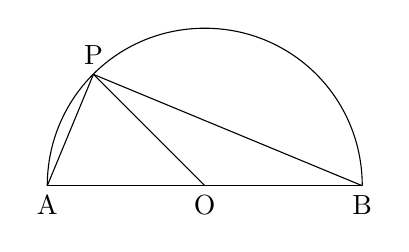
\begin{tikzpicture}
  [help lines/.style={dashed}]
  \draw (-2, 0) .. controls (-2, 1.11) and (-1.11, 2) .. (0, 2)
                .. controls (1.11, 2) and (2, 1.11) .. (2, 0);
  \draw[-] (-2, 0) node[anchor=north]{A} -- (2, 0) node[anchor=north]{B};
  \draw[-] (-1.414, 1.414) node[anchor=south]{P} -- (-2, 0);
  \draw[-] (-1.414, 1.414) -- (2, 0);
  \draw[-] (-1.414, 1.414) -- (0, 0) node[anchor=north]{O};
\end{tikzpicture}

Suppose $P$ is a random point on the semicircle, then $APB$ is an angle 
inscribed in a semicircle.
\begin{equation*}
\begin{split}
  \vec{PA} \cdot \vec{PB} &= (\vec{OA} - \vec{OP}) \cdot (\vec{OB} - \vec{OP}) \\
                          &= \vec{OA} \cdot \vec{OB} + |\vec{OP}|^2 - \vec{OA} \cdot \vec{OP} - \vec{OB} \cdot \vec{OP} \\
                          &= -|\vec{OA}|^2 + |\vec{OP}|^2 - (\vec{OA} + \vec{OB}) \cdot \vec{OP} \\
\end{split}
\end{equation*}
Given that $APB$ is inscribed in a semicircle, 
$|\vec{OA}| = |\vec{OB}| = |\vec{OP}|$, and $\vec{OA} = -\vec{OB}$.
\begin{gather*}
  \begin{split}
    \vec{PA} \cdot \vec{PB} &= -|\vec{OA}|^2 + |\vec{OP}|^2 - (\vec{OA} + \vec{OB}) \cdot \vec{OP} \\ 
                            &= -|\vec{OP}|^2 + |\vec{OP}|^2 - \vec{0} \cdot \vec{OP} \\
                            &= 0 \\
  \end{split} \\
  \vec{PA} \perp \vec{PB}
\end{gather*}
Therefore, it is proved that an angle inscribed in a semicircle is a right 
angle.

8. Prove the trigonometric formula: 
$\cos(\theta_1 - \theta_2) = \cos\theta_1\cos\theta_2 + \sin\theta_1\sin\theta_2$.

Proof:

Suppose the angle between the unit vector $\vec{u_1}$ and $\vec{i}$ is 
$\theta_1$, and the angle between the unit vector $\vec{u_2}$ and $\vec{i}$ is 
$\theta_2$.
\begin{gather*}
  \vec{u_1} = <\cos\theta_1, \sin\theta_1> \\
  \vec{u_2} = <\cos\theta_2, \sin\theta_2> \\
\end{gather*}
The angle between $\vec{u_1}$ and $\vec{u_2}$ is $|\theta_1 - \theta_2|$. Hence,
\begin{gather*}
  \begin{split}
    \vec{u_1} \cdot \vec{u_2} &= |\vec{u_1}| \cdot |\vec{u_2}| \cdot \cos(|\theta_1 - \theta_2|) \\
                              &= |\vec{u_1}| \cdot |\vec{u_2}| \cdot \cos(\theta_1 - \theta_2) \\
                              &= \cos(\theta_1 - \theta_2) \\
  \end{split} \\
  \begin{split}
    \vec{u_1} \cdot \vec{u_2} &= <\cos\theta_1, \sin\theta_1> \cdot <\cos\theta_2, \sin\theta_2> \\
                              &= \cos\theta_1\cos\theta_2 + \sin\theta_1\sin\theta_2 \\
  \end{split} \\
  \cos(\theta_1 - \theta_2) = \cos\theta_1\cos\theta_2 + \sin\theta_1\sin\theta_2 \\
\end{gather*}

Therefore, it is proved that 
$\cos(\theta_1 - \theta_2) = \cos\theta_1\cos\theta_2 + \sin\theta_1\sin\theta_2$.

\subsection*{Unit 3 Determinants}

1. Calculate the value of the determinants\\
a) $\begin{vmatrix}
    1 & 4 \\
    2 & -1 \\
\end{vmatrix}$

b) $\begin{vmatrix}
    3 & -4 \\
    -1 & -2 \\
\end{vmatrix}$

Solution:

a)
\[
  \begin{vmatrix}
    1 & 4 \\
    2 & -1 \\
  \end{vmatrix} = (1 \times (-1)) - (4 \times 2) = -9
\]

b)
\[
  \begin{vmatrix}
    3 & -4 \\
    -1 & -2 \\
  \end{vmatrix} = (3 \times (-2)) - ((-4) \times (-1)) = -10
\]

2. Calculate 
$\begin{vmatrix}
  -1 & 0 & 4 \\
  1 & 2 & 2 \\
  3 & -2 & -1 \\
\end{vmatrix}$ using the Laplace expansion by the cofactors of:\\
a) the first row \hspace{10px} b) the first column

Solution:

a)
\begin{equation*}
\begin{split}
  \begin{vmatrix}
    -1 & 0 & 4 \\
    1 & 2 & 2 \\
    3 & -2 & -1 \\
  \end{vmatrix} 
  &= (-1) \cdot \begin{vmatrix}
                  2 & 2 \\
                  -2 & -1 \\ 
                \end{vmatrix} -
     0 \cdot \begin{vmatrix}
               1 & 2 \\
               3 & -1 \\ 
             \end{vmatrix} +
     4 \cdot \begin{vmatrix}
               1 & 2 \\
               3 & -2 \\ 
             \end{vmatrix} \\ 
  &= (-1) \times 2 - 0 \times (-7) + 4 \times (-8) \\
  &= -34 \\
\end{split}
\end{equation*}

b)
\begin{equation*}
\begin{split}
  \begin{vmatrix}
    -1 & 0 & 4 \\
    1 & 2 & 2 \\
    3 & -2 & -1 \\
  \end{vmatrix} 
  &= (-1) \cdot \begin{vmatrix}
                  2 & 2 \\
                  -2 & -1 \\ 
                \end{vmatrix} -
     1 \cdot \begin{vmatrix}
               0 & 4 \\
               -2 & -1 \\ 
             \end{vmatrix} +
     3 \cdot \begin{vmatrix}
               0 & 4 \\
               2 & 2 \\ 
             \end{vmatrix} \\ 
  &= (-1) \times 2 - 1 \times (8) + 3 \times (-8) \\
  &= -34 \\
\end{split}
\end{equation*}

3. Find the area of the plane triangle whose vertices lie at\\
a) $(0, 0), (1, 2), (1, -1)$ \hspace{10px} b) $(1, 2), (1, -1), (2, 3)$

Solution:

a) The vectors of the two edges of the plane triangle are $<1, 2>$ and 
$<1, -1>$. The area of the plane triangle $A$ can be calculated as
\begin{gather*}
  \begin{split}
    det(<1, 2>, <1, -1>) &= \begin{vmatrix}
                              1 & 2 \\
                              1 & -1 \\ 
                            \end{vmatrix} \\
                         &= -3
  \end{split} \\
  A = |det(<1, 2>, <1, -1>)| = 3 \\
\end{gather*}

b) The vectors of the two edges of the plane triangle are $<0, -3>$ and 
$<1, 1>$. The area of the plane triangle $A$ can be calculated as
\begin{gather*}
  \begin{split}
    det(<0, -3>, <1, 1>) &= \begin{vmatrix}
                              0 & -3 \\
                              1 & 1 \\ 
                            \end{vmatrix} \\
                         &= 3
  \end{split} \\
  A = |det(<1, 2>, <1, -1>)| = 3 \\
\end{gather*}

4. a) Show that the value of a $2 \times 2$ determinants is unchanged if you add
to the second row a scalar multiple of the first row.\\
   b) Show that the value of a $2 \times 2$ determinants is unchanged if you add
to the second column a scalar multiple of the first column.

Solution:

a)
\begin{gather*}
  \begin{vmatrix}
    a_1 & a_2 \\
    b_1 & b_2 \\
  \end{vmatrix} = a_1b_2 - a_2b_1 \\
  \begin{split}
    \begin{vmatrix}
      a_1 & a_2 \\
      b_1 + c \cdot a_1 & b_2 + c \cdot a_2 \\
    \end{vmatrix} &= 
    a_1 \cdot (b_2 + c \cdot a_2) - a_2 \cdot (b_1 + c \cdot a_1) \\
    &= a_1b_2 + c \cdot a_1a_2 - a_2b_1 - c \cdot a_1a_2 \\
    &= a_1b_2 - a_2b_1 \\
  \end{split} \\
\end{gather*}

b)
\begin{gather*}
  \begin{vmatrix}
    a_1 & a_2 \\
    b_1 & b_2 \\
  \end{vmatrix} = a_1b_2 - a_2b_1 \\
  \begin{split}
    \begin{vmatrix}
      a_1 & c \cdot a_1 + a_2 \\
      b_1 & c \cdot b_1 + b_2 \\
    \end{vmatrix} &= 
    a_1 \cdot (c \cdot b_1 + b_2) - b_1 \cdot (c \cdot a_1 + a_2) \\
    &= c \cdot a_1b_1 + a_1b_2 - c \cdot a_1b_1 - a_2b_1\\
    &= a_1b_2 - a_2b_1 \\
  \end{split} \\
\end{gather*}

5. Use a Laplace expansion and Exercise 4a to show the value of a $3 \times 3$
determinants is unchanged if you add to the second row a scalar multiple of the
third row.

Solution:

\begin{gather*}
  \begin{vmatrix}
    a_1 & a_2 & a_3 \\
    b_1 & b_2 & b_3 \\
    c_1 & c_2 & c_3 \\
  \end{vmatrix} = 
  a_1 \cdot \begin{vmatrix}
              b_2 & b_3 \\
              c_2 & c_3 \\ 
            \end{vmatrix} -
  a_2 \cdot \begin{vmatrix}
              b_1 & b_3 \\
              c_1 & c_3 \\
            \end{vmatrix} + 
  a_3 \cdot \begin{vmatrix}
              b_1 & b_2 \\
              c_1 & c_2 \\ 
            \end{vmatrix} \\
  \begin{vmatrix}
    a_1 & a_2 & a_3 \\
    b_1 + k \cdot c_1 & b_2 + k \cdot c_2 & b_3 + k \cdot c_3 \\
    c_1 & c_2 & c_3 \\
  \end{vmatrix} = 
  a_1 \cdot \begin{vmatrix}
              b_2 + k \cdot c_2 & b_3 + k \cdot c_3 \\
              c_2 & c_3 \\ 
            \end{vmatrix} - \\
  a_2 \cdot \begin{vmatrix}
              b_1 + k \cdot c_1 & b_3 + k \cdot c_3 \\
              c_1 & c_3 \\
            \end{vmatrix} + 
  a_3 \cdot \begin{vmatrix}
              b_1 + k \cdot c_1 & b_2 + k \cdot c_2 \\
              c_1 & c_2 \\ 
            \end{vmatrix} \\
\end{gather*}
According to the result of Exercise 4a,
\begin{gather*}
  \begin{vmatrix}
    b_2 + k \cdot c_2 & b_3 + k \cdot c_3 \\
    c_2 & c_3 \\ 
  \end{vmatrix} = 
  \begin{vmatrix}
    b_2 & b_3 \\
    c_2 & c_3 \\ 
  \end{vmatrix} \\
  \begin{vmatrix}
    b_1 + k \cdot c_1 & b_3 + k \cdot c_3 \\
    c_1 & c_3 \\ 
  \end{vmatrix} = 
  \begin{vmatrix}
    b_1 & b_3 \\
    c_1 & c_3 \\ 
  \end{vmatrix} \\
  \begin{vmatrix}
    b_1 + k \cdot c_1 & b_2 + k \cdot c_2 \\
    c_1 & c_2 \\ 
  \end{vmatrix} = 
  \begin{vmatrix}
    b_1 & b_2 \\
    c_1 & c_2 \\ 
  \end{vmatrix} \\
\end{gather*}
Therefore,
\begin{equation*}
\begin{split}
  \begin{vmatrix}
    a_1 & a_2 & a_3 \\
    b_1 + k \cdot c_1 & b_2 + k \cdot c_2 & b_3 + k \cdot c_3 \\
    c_1 & c_2 & c_3 \\
  \end{vmatrix} 
  &= a_1 \cdot \begin{vmatrix}
                 b_2 + k \cdot c_2 & b_3 + k \cdot c_3 \\
                 c_2 & c_3 \\ 
               \end{vmatrix} -
     a_2 \cdot \begin{vmatrix}
                 b_1 + k \cdot c_1 & b_3 + k \cdot c_3 \\
                 c_1 & c_3 \\
               \end{vmatrix} + \\
     a_3 \cdot \begin{vmatrix}
                 b_1 + k \cdot c_1 & b_2 + k \cdot c_2 \\
                 c_1 & c_2 \\ 
               \end{vmatrix} \\
  &= a_1 \cdot \begin{vmatrix}
                 b_2 & b_3 \\
                 c_2 & c_3 \\ 
               \end{vmatrix} -
     a_2 \cdot \begin{vmatrix}
                 b_1 & b_3 \\
                 c_1 & c_3 \\
               \end{vmatrix} + 
     a_3 \cdot \begin{vmatrix}
                 b_1 & b_2 \\
                 c_1 & c_2 \\ 
               \end{vmatrix} \\
  &= \begin{vmatrix}
       a_1 & a_2 & a_3 \\
       b_1 & b_2 & b_3 \\
       c_1 & c_2 & c_3 \\
     \end{vmatrix} \\
\end{split}
\end{equation*}

6. Let $(x_{1}, y_{1})$ and $(x_{2}, y_{2})$ both range over all unit vectors.
Find the maximum value of the function $f(x_{1}, x_{2}, y_{1}, y_{2}) =
\begin{vmatrix}
x_{1} & y_{1} \\
x_{2} & y_{2} \\
\end{vmatrix}$.

Solution:

According to the geometric interpretation of $2 \times 2$ determinants, the 
value of the function $f(x_{1}, x_{2}, y_{1}, y_{2}) =
\begin{vmatrix}
x_{1} & y_{1} \\
x_{2} & y_{2} \\
\end{vmatrix}$ is the positive or negative value of the parallelogram formed by 
the two unit vectors $(x_1, y_1)$ and $(x_2, y_2)$. The area of the 
parallelogram formed by these two vectors can be calculated as
\begin{equation*}
\begin{split}
  A &= |<x_1, y_1>| \cdot |<x_2, y_2>| \cdot \sin\theta \\
    &= \sin\theta \\
\end{split}
\end{equation*}
where $\theta$ is the angle between these two vectors.

Apparently, the maximum value of the area of the parallelogram formed by these 
two vectors is $1$, which is achieved when $\theta = \frac{\pi}{2}$, i.e. the 
two unit vectors are perpendicular to each other.

\subsection*{Unit 4 Cross Product}

1. Find $\vec{A} \times \vec{B}$ if\\
a) $\vec{A} = \vec{i} - 2 \vec{j} + \vec{k}$, $\vec{B} = 2 \vec{i} - \vec{j} -
\vec{k}$ \\
b) $\vec{A} = 2 \vec{i} - 3 \vec{k}$, $\vec{B} = \vec{i} + \vec{j} - \vec{k}$

Solution:

a)
\begin{equation*}
\begin{split}
  \vec{A} \times \vec{B} 
  &= \begin{vmatrix}
       \vec{i} & \vec{j} & \vec{k} \\
       1 & -2 & 1 \\
       2 & -1 & -1 \\
     \end{vmatrix} \\
  &= \vec{i} \cdot \begin{vmatrix}
                     -2 & 1 \\
                     -1 & -1 \\
                   \end{vmatrix} - 
     \vec{j} \cdot \begin{vmatrix}
                     1 & 1 \\
                     2 & -1 \\    
                   \end{vmatrix} + 
     \vec{k} \cdot \begin{vmatrix}
                     1 & -2 \\
                     2 & -1 \\ 
                   \end{vmatrix} \\
  &= 3\vec{i} + 3\vec{j} + 3\vec{k} \\
\end{split}
\end{equation*}

b)
\begin{equation*}
\begin{split}
  \vec{A} \times \vec{B} 
  &= \begin{vmatrix}
       \vec{i} & \vec{j} & \vec{k} \\
       2 & 0 & -3 \\
       2 & 1 & -1 \\
     \end{vmatrix} \\
  &= \vec{i} \cdot \begin{vmatrix}
                     0 & -3 \\
                     1 & -1 \\
                   \end{vmatrix} - 
     \vec{j} \cdot \begin{vmatrix}
                     2 & -3 \\
                     2 & -1 \\    
                   \end{vmatrix} + 
     \vec{k} \cdot \begin{vmatrix}
                     2 & 0 \\
                     2 & 1 \\ 
                   \end{vmatrix} \\
  &= 3\vec{i} - 4\vec{j} + 2\vec{k} \\
\end{split}
\end{equation*}

2. Find the area of the triangle in space having its vertices at the points
\[ P:(2,0,1), Q:(3,1,0), R:(-1,1,-1).\]

Solution:

\begin{gather*}
  \vec{PQ} = <1, 1, -1> \\
  \vec{PR} = <-3, 1, -2> \\
  \begin{split}
    \vec{PQ} \times \vec{PR} 
    &= \begin{vmatrix}
         \vec{i} & \vec{j} & \vec{k} \\
         1 & 1 & -1 \\
         -3 & 1 & -2 \\
       \end{vmatrix} \\
    &= <-1, 5, 4> \\
  \end{split} \\
  \begin{split}
    A &= \frac{|\vec{PQ} \times \vec{PR}|}{2} \\
      &= \frac{\sqrt{(-1)^2 + 5^2 + 4^2}}{2} \\
      &= \frac{\sqrt{42}}{2} \\
  \end{split} \\
\end{gather*}
Therefore, the area of the described triangle is $\frac{\sqrt{42}}{2}$.

3. Two vectors $\vec{i'}$ and $\vec{j'}$ of a right-handed coordinate system are 
to have the directions respectively of the vectors $\vec{A} = 2\vec{i} - \vec{j}$ 
and $\vec{B} = \vec{i} + 2\vec{j} + \vec{k}$. Find all three vectors
$\vec{i'}$, $\vec{j'}$, $\vec{k'}$.

Solution:

According to the problem description, $\vec{i'}$ is the direction of the vector 
$\vec{A} = 2\vec{i} - \vec{j}$, hence
\begin{equation*}
\begin{split}
  \vec{i'} &= \frac{\vec{A}}{|\vec{A}|} \\
           &= \frac{<2, -1, 0>}{\sqrt{5}} \\
           &= <\frac{2\sqrt{5}}{5}, -\frac{\sqrt{5}}{5}, 0> \\
\end{split}
\end{equation*}

Similarly, since $\vec{j'}$ is the direction of the vector 
$\vec{B} = \vec{i} + 2\vec{j} + \vec{k}$,
\begin{equation*}
\begin{split}
  \vec{j'} &= \frac{\vec{B}}{|\vec{B}|} \\
           &= \frac{<1, 2, 1>}{\sqrt{6}} \\
           &= <\frac{\sqrt{6}}{6}, \frac{2\sqrt{6}}{6}, \frac{\sqrt{6}}{6}> \\
\end{split}
\end{equation*}
According to the geometric interpretation of cross product,
\begin{gather*}
  \begin{split}
    \vec{A} \times \vec{B}
    &= \begin{vmatrix}
         \vec{i} & \vec{j} & \vec{k} \\
         2 & -1 & 0 \\
         1 & 2 & 1 \\
       \end{vmatrix} \\
    &= <-1, -2, 5>
  \end{split} \\
  \begin{split}
    \vec{k'} &= dir(\vec{A} \times \vec{B}) \\
             &= \frac{\vec{A} \times \vec{B}}{|\vec{A} \times \vec{B}|} \\
             &= \frac{<-1, -2, 5>}{\sqrt{30}} \\
             &= <-\frac{\sqrt{30}}{30}, -\frac{\sqrt{30}}{15}, \frac{\sqrt{30}}{6}> \\
  \end{split}
\end{gather*}

4. Verify that the cross product $\times$ does not in general satisfy the
associative law, by showing that for the particular vectors $\vec{i}$,
$\vec{j}$, $\vec{k}$, we have $(\vec{i} \times \vec{j}) \times \vec{k} \neq
\vec{i} \times (\vec{j} \times \vec{k})$.

Solution:

Suppose that $\vec{i} = <1, 0, 1>$, $\vec{j} = <1, 1, 0>$, and 
$\vec{k} = <0, 1, 1>$.
Then
\begin{gather*}
  (\vec{i} \times \vec{j}) \times \vec{k} = <0, 1, -1> \\
  \vec{i} \times (\vec{j} \times \vec{k}) = <1, 0, -1> \\
\end{gather*}
Hence, the cross product does not in general satisfy the associative law.

5. What can you conclude about $\vec{A}$ and $\vec{B}$\\
a) if $|\vec{A} \times \vec{B}| = |\vec{A}| |\vec{B}|$;\\
b) if $|\vec{A} \times \vec{B}| = \vec{A} \cdot \vec{B}$.

Solution:

a) According to the geometric interpretation of cross product, 
$|\vec{A} \times \vec{B}|$ is the area of the parallelogram formed by the 
vectors $\vec{A}$ and $\vec{B}$. Therefore,
\[
  |\vec{A} \times \vec{B}| = |\vec{A}| |\vec{B}| \sin\theta
\]
where $\theta$ is the angle between the vectors $\vec{A}$ and $\vec{B}$.

Then if $|\vec{A} \times \vec{B}| = |\vec{A}| |\vec{B}|$,
\begin{gather*}
  |\vec{A} \times \vec{B}| = |\vec{A}| |\vec{B}| \\
  |\vec{A}| |\vec{B}| \sin\theta = |\vec{A}| |\vec{B}| \\
  \sin\theta = 1 \\
  \theta = \frac{\pi}{2} \\
\end{gather*}
We can conclude that the angle between the vectors $\vec{A}$ and $\vec{B}$ is 
$\frac{\pi}{2}$.

b) Similar to Exercise a), if 
$|\vec{A} \times \vec{B}| = \vec{A} \cdot \vec{B}$,
\begin{gather*}
  |\vec{A} \times \vec{B}| = \vec{A} \cdot \vec{B} \\
  |\vec{A}| |\vec{B}| \sin\theta = |\vec{A}| |\vec{B}| \cos\theta \\
  \sin\theta = \cos\theta \\
  \theta = \frac{pi}{4} \\
\end{gather*}
We can conclude that the angle between the vectors $\vec{A}$ and $\vec{B}$ is 
$\frac{\pi}{4}$.

6. Find the volume of the tetrahedron having vertices at the four points
\[ P:(1,0,1), Q:(-1,1,2), R:(0,0,2), S:(3,1,-1).\]

Solution:

\begin{gather*}
  \vec{PQ} = <-2, 1, 1> \\
  \vec{PR} = <-1, 0, 1> \\
  \vec{PS} = <2, 1, -2> \\
\end{gather*}

According to the geometric interpretation of $3 \times 3$ determinants, the 
volume of the tetrahedron with the described vertices can be calculated as
\begin{gather*}
  \begin{split}
    det(\vec{PQ}, \vec{PR}, \vec{PS}) 
    &= \begin{vmatrix}
         -2 & 1 & 1 \\
         -1 & 0 & 1 \\
         2 & 1 & -2 \\
       \end{vmatrix} \\
    &= -2 \times (-1) - 1 \times 0 + 1 \times (-1) \\
    &= 1
  \end{split} \\
  \begin{split}
    V &= |det(\vec{PQ}, \vec{PR}, \vec{PS})| \\
      &= 1 \\
  \end{split} \\
\end{gather*}
Therefore, the volume of the described tetrahedron is 1.

\begin{center}
\section*{Part II}
\end{center}

1. Find the dihedral angle between two faces of a regular tetrahedron.

Solution:

\begin{definition}
  A dihedral angle is the angle between two intersecting planes or half-planes.
\end{definition}

\begin{definition}
  A regular tetrahedron is a tetrahedron in which all four faces are equilateral 
  triangles.
\end{definition}

\begin{definition}
  In geometry, an equilateral triangle is a triangle in which all three sides 
  have the same length.
\end{definition}

\begin{tikzpicture}
  [help line/.style={dashed}]
  \draw[->] (-3, 0, 0) -- (3, 0, 0) node[below right] {x};
  \draw[->] (0, -1, 0) -- (0, 3, 0) node[right] {y};
  \draw (0, 0) node[below right] {O};
  \draw[-] (-1, 0, 0) -- (1, 0, 0);
  \draw[-] (-1, 0, 0) -- (0, 1.732, 0);
  \draw[-] (1, 0, 0) -- (0, 1.732, 0);
  \draw (0, 1.732) node[above] {A};
  \draw (-1, 0) node[left] {B};
  \draw (1, 0) node[right] {C};
  \draw[help line] (0, 1.732, 0) -- (0, 0, 0);
  \draw[help line] (-1, 0, 0) -- (0.5, 0.866, 0);
  \draw[help line] (1, 0, 0) -- (-0.5, 0.866, 0);
  \draw (0, 0.577) node[below right] {S'};
\end{tikzpicture}

Suppose that there is a regular tetrahedron whose length is 2. Let A, B, C, S 
denote the four vertices of the tetrahedron, and we'll build a Cartesian 
coordinate system as shown in the diagram.

According to the geometric property of a regular tetrahedron, we can get 
the coordinates of the four vertices:
\[ A = (0, \sqrt{3}, 0), B = (-1, 0, 0), C = (1, 0, 0), S = (0, \frac{\sqrt{3}}{3}, \frac{2\sqrt{3}}{3})\]

To calculate the dihedral angle between two planes, we can find a point on the 
intersection line, and from that point find two lines in two planes respectively 
which is perpendicular to the intersection line. 

In this case, we 'll try to find the dihedral angle between the plane $ABC$ and 
$SBC$, using the point $O$ as the starting point and hence $BC$ as the 
intersection line. According to the geometric property of equilateral triangles:
\[ OA \perp BC, OS \perp BC \]
Therefore, the dihedral angle between the plane $ABC$ and $SBC$ is the angle 
$\angle{AOS}$ between the line $OA$ and $OS$.
\begin{gather*}
  \vec{OA} = <0, \sqrt{3}, 0> \\
  \vec{OS} = <0, \frac{\sqrt{3}}{3}, \frac{2\sqrt{3}}{3}> \\
  \begin{split}
    \cos\angle{AOS} &= \frac{\vec{OA} \cdot \vec{OS}}{|\vec{OA}| \cdot |\vec{OS}|} \\
                    &= \frac{0 \times 0 + \sqrt{3} \times \frac{\sqrt{3}}{3} + 0 \times \frac{2\sqrt{3}}{3}}{\sqrt{3} \times \sqrt{(\frac{\sqrt{3}}{3})^2 + (\frac{2\sqrt{3}}{3})^2}} \\
                    &= \frac{\sqrt{5}}{5} \\
  \end{split} \\
  \angle{AOS} = cos^{-1}(\frac{\sqrt{5}}{5}) \\
\end{gather*}
Therefore, the dihedral angle between two faces of a regular tetrahedron is 
$cos^{-1}(\frac{\sqrt{5}}{5})$.

2. a) Show that the 'polarization identity'
$\frac{1}{4}(|\vec{u} + \vec{v}|^{2} - |\vec{u} - \vec{v}|^{2}) = \vec{u} \cdot \vec{v}$ 
holds for any two n-vectors $\vec{u}$ and $\vec{v}$. (Use vector algebra, not 
components.) \\
b) Given two non-zero vectors $\vec{u}$ and $\vec{v}$, give the formula for the
unit vector which bisects the (smaller) angle between $\vec{u}$ and $\vec{v}$.
(Use the notation $\hat{\vec{u}}$ for the unit vector in the $\vec{u}$ -
direction.)

Solution:

a) Proof:
\begin{gather*}
  \begin{split}
    \frac{1}{4}(|\vec{u} + \vec{v}|^{2} - |\vec{u} - \vec{v}|^{2}) &= \frac{1}{4}((\vec{u} + \vec{v})^2 - (\vec{u} - \vec{v})^2) \\
                                                                   &= \frac{1}{4}((\vec{u}^2 + \vec{v}^2 + 2\vec{u} \cdot \vec{v}) - (\vec{u}^2 + \vec{v}^2 - 2\vec{u} \cdot \vec{v})) \\
                                                                   &= \frac{1}{4}(4\vec{u} \cdot \vec{v}) \\
                                                                   &= \vec{u} \cdot \vec{v} \\
  \end{split} \\
\end{gather*}

b) According to the geometric interpretation of the addition of vectors, for two 
unit vectors $\vec{a}$ and $\vec{b}$, the vector $\vec{a} + \vec{b}$ bisects the 
(smaller) angle between $\vec{a}$ and $\vec{b}$ because $\vec{a}$, $\vec{b}$, 
and $\vec{a} + \vec{b}$ would form an isosceles triangle where the $\vec{a}$ and 
$\vec{b}$ are the two side that have equal lengths.

Therefore, to find the unit vector which bisects the (smaller) angle between 
$\vec{u}$ and $\vec{v}$, we can find the unit vector which bisects the (smaller) 
angle between $\hat{\vec{u}}$ and $\hat{\vec{v}}$, which is
\begin{gather*}
  \begin{split}
    \vec{w} &= \frac{\hat{\vec{u}} + \hat{\vec{v}}}{|\hat{\vec{u}} + \hat{\vec{v}}|} \\
            &= \frac{\frac{\vec{u}}{|\vec{u}|} + \frac{\vec{v}}{|\vec{v}|}}{\sqrt{(\frac{\vec{u}}{|\vec{u}|} + \frac{\vec{v}}{|\vec{v}|})^2}} \\
            &= \frac{\frac{|\vec{v}| \cdot \vec{u} + |\vec{u}| \cdot \vec{v}}{|\vec{u}| \cdot |\vec{v}|}}{\sqrt{2 + 2\frac{\vec{u} \cdot \vec{v}}{|\vec{u} \cdot |\vec{v}|}}} \\
            &= \frac{|\vec{v}| \cdot \vec{u} + |\vec{u}| \cdot \vec{v}}{\sqrt{2|\vec{u}|^2 \cdot |\vec{v}|^2 + 2|\vec{u}||\vec{v}|\vec{u} \cdot \vec{v}}}
  \end{split} \\
\end{gather*}

3. In this problem we examine tacking, which is the process sailboats use to
travel against the wind. Sails are a familar tool to harness the energy of the
wind for transportation over the sea. Early ships had large fixed sails which
would capture the wind blowing from behind to propel the ship forward. Even if
the wind is blowing behind at an (acute) angle the component of the wind vector
perpendicular to the sail will push on the sail and hence on the boat. However,
these early fixed sail ships had no way to go against the wind and had to rely
on oarsmen if the wind was blowing in the wrong direction.

A great advance that allowed boats to sail against the wind was the invention
of movable sails in combination with a rudder and a keel. By carefully
positioning the sail the boat can be made to sail into the wind - this process
is called \emph{tacking}.

As noted before, the component of the wind perpendicular to the sail pushes on
the sail and, through it, the boat. The keel only allows the boat to move along
its axis. (The rudder is used to turn the boat.) That is, for any force on the
boat, only the component along the boat's axis actually pushes the boat.

Described mathematically, the wind vector is first projected on the
perpendicular to the sail to get the direction of the force on the sail. This
resultant force is projected on the axis of the boat to find the direction the
boat is being pushed. By orienting the sail correctly this double projection
can result in a vector with a component pointing into the wind.

\begin{tikzpicture}
  [help line/.style={dashed}]
  \draw[help line] (-3, 0, 0) -- (3, 0, 0) node[right] {x};
  \draw[help line] (0, -3, 0) -- (0, 3, 0) node[above] {y};
  \draw[->] (0, 0, 0) -- (2, 0, 0) node[below] {$\vec{w} = a\vec{i}$};
  \draw[-] (-1, -1.732, 0) -- (1, 1.732, 0) node[above right] {$l_s$};
  \draw[-] (1, -1.732, 0) -- (-1, 1.732, 0) node[above left] {$l_B$};
  \draw (0, 0, 0) node[above right] {$\alpha$};
  \draw (0, 0, 0) node[above] {$\beta$};
\end{tikzpicture}

In the picture $\vec{w} = a \vec{i}$ is the wind direction. The line $l_s$ is 
perpendicular to the sail (with $0 \leq \alpha \leq \frac{\pi}{2}$). And the 
line $l_B$ is along the boat's axis (with $0 \leq \beta \leq \frac{\pi}{2}$).

a) Let $\vec{w_1}$ be the projection of $\vec{w}$ onto the line $l_s$. Show that 
$\vec{w_1}$ does not have a non-zero component in the direction opposite 
$\vec{w}$. (It is sufficient to show the projections on the sketch.)

b) Find the projection of $\vec{w_{1}}$ onto $l_{B}$. (Give an explicit formula
in terms of $\alpha$ and $\beta$.) What is the condition on $\alpha$ and $\beta$
that this projection has a component in the $-\vec{i}$ direction? (For warmup
you might try the specific case $\alpha = \frac{\pi}{3} = \beta$.)

Solution:

a) According to the definition of additions and decomposition of vectors, the 
projection $\vec{w_1}$ of $\vec{w}$ along the line $l_s$ must have an acute 
angle, which is $\alpha$, with $\vec{w}$. Therefore, $\vec{w_1}$ has an obtuse 
angle with the reverse direction of $\vec{w}$. Therefore, according to the rule 
of vector decomopsition, $\vec{w_1}$ cannot have a non-zero component on the 
reverse direction of $\vec{w}$. 

b) Let $\vec{w_B}$ denote the projection vector of $\vec{w_1}$ onto $l_B$. Then
\begin{gather*}
  \begin{split}
    |\vec{w_B}| &= |\vec{w_1}| \cos\beta \\
                &= |\vec{w}| \cos\alpha \cos\beta \\
                &= a \cos\alpha \cos\beta \\
  \end{split} \\
\end{gather*}
From geometric point of view, for the projection of $\vec{w_B}$ on the x axis, 
we can see from the diagram that if $l_B$ passes the second quadrant, 
$\vec{w_B}$ would has a non-zero component along the reverse direction of 
$\vec{i}$. Therefore, the condition is that $\alpha + \beta > \frac{\pi}{2}$.

From analytical point of view, the component of $\vec{w_B}$ on the $-\vec{i}$ 
direction can be calculated as
\begin{gather*}
  \begin{split}
    |\vec{w_B}| \cos(\pi - \alpha - \beta) = -|\vec{w_B}| \cos(\alpha + \beta)
  \end{split}
\end{gather*}
Therefore, to make sure the component on the $-\vec{i}$ direction is non-zero, 
the condition is:
\begin{itemize}
  \item $|\vec{w_B}|$ is non-zero, which is guaranteed by the values of $a$, 
    $\alpha$ and $\beta$.
  \item $\cos(\alpha + \beta) < 0$, which is equivalent to 
    $\alpha + \beta > \frac{\pi}{2}$.
\end{itemize}

\end{document}